
\chapter{Functional-structural Plant Models} \label{chapter:fspm}

This chapter looks at current developments in the field of \textit{in silico} plants, intending to design \acrshort{rc} experiments with simulated organisms.
Research with \textit{in vivo} plants is difficult and time-consuming as it involves meticulous experimental design, long observation times, and of course keeping the plants healthy during the experiment\citep{pieters_plants_2021}.
For these reasons, it is of great interest to explore computer simulations of plants that can accelerate research in reservoir computing applications.
 \label{fspm:why}

% \section{Selection criteria for RC experiments}
\section{Selecting Plant Models for RC Experiments} \label{fspm:selecting-models-for-rc}


% Types of plant models
% Plant models exist in many shapes and sizes. 
There exist many different types of plant models.
To get an idea of the various model categories one can visit \textit{Quantitative Plant}\footnote[1]{https://www.quantitative-plant.org/model. See \citet{lobet_online_2013, lobet_image_2017} for more details.}, 
a website that aggregates open-source plant models from the literature.
Listed models range from crop surface models (\acrshort{csm}) that estimate biomass and crop yield from aerial imagery \citep{tilly_multitemporal_2014} to sub-plant models that simulate gas exchange between the canopy and the environment \citep{sinoquet_ratp_2001}.

%%% TODO %%%

% Selection criteria: single organism
To select plant models for use in \acrshort{rc} experiments, they must meet certain criteria. 
Firstly, the model must track the state of a single plant over time, 
as the scope of the research presented limits the interpretation of the reservoir to a single organism.
This rules out the use of e.g.\ crop surface models because they only inform about large populations of plants; in these models information on the level of an individual organism is lost (although it would certainly be interesting to apply reservoir computing principles to the ecological dynamics of a crop field).


% Selection criteria: 3d anatomy
Secondly, the plant's state should be observable from multiple fixed points of the plant's anatomy. 
These observed points must be distinct structural elements of the plant that simulate the physiological processes of a real specimen and must communicate with one another as a dynamical system.
We set this requirement because an RC system using a plant model as reservoir is intended to represent the equivalent setup in the real world.
This requirement entails a preference for mechanistic models that make few prior assumptions about plant behavior, leaving macroscopic behavior to emerge naturally from microscopic interactions at the cellular level \citep{gauthier_functional_2020}.
Ideally, the observable parameters of the plant are also empirically measurable \textit{in vivo} to enable the research results from this work to be better transferable to a real-world setting.


% Selection criteria: time resolution
Finally, the time resolution of the simulation should be sufficiently fine to observe dynamics at multiple time scales as well as avoid signal aliasing (see \mbox{Section \ref{section:rc-time-scales}}).

 

\section{Functional-structural Plant Models (FSPMs)} \label{fspm:fspm-intro}


% What are \acrshort{fspm}s?
A promising category of models that can the stated criteria is that of functional-structural plant models (\acrshort{fspm}) \citep{godin_functionalstructural_2005, louarn_two_2020}.
\acrshort{fspm} model the plant as a collection of interconnected units that represent a small structural part of the plant in space.
These units interact with the environment and with each other to simulate eco-physiological processes \citep{coussement_turgor-driven_2020}. 
The structural elements of the simulated plant form a hierarchy of interactions at different scales. Together they govern the macroscopic behavior of the organism \citep{louarn_two_2020}. Most \acrshort{fspm}s simulate interactions across a range of scales, from cell organelles to whole plant organs and even populations of multiple organisms. A schematic representation of the different scales of interactions is shown on Figure \ref{fig:fspm_scales_louarn2020}.

\begin{figure}[t]
	\centering
% 	\copyrightbox[r]{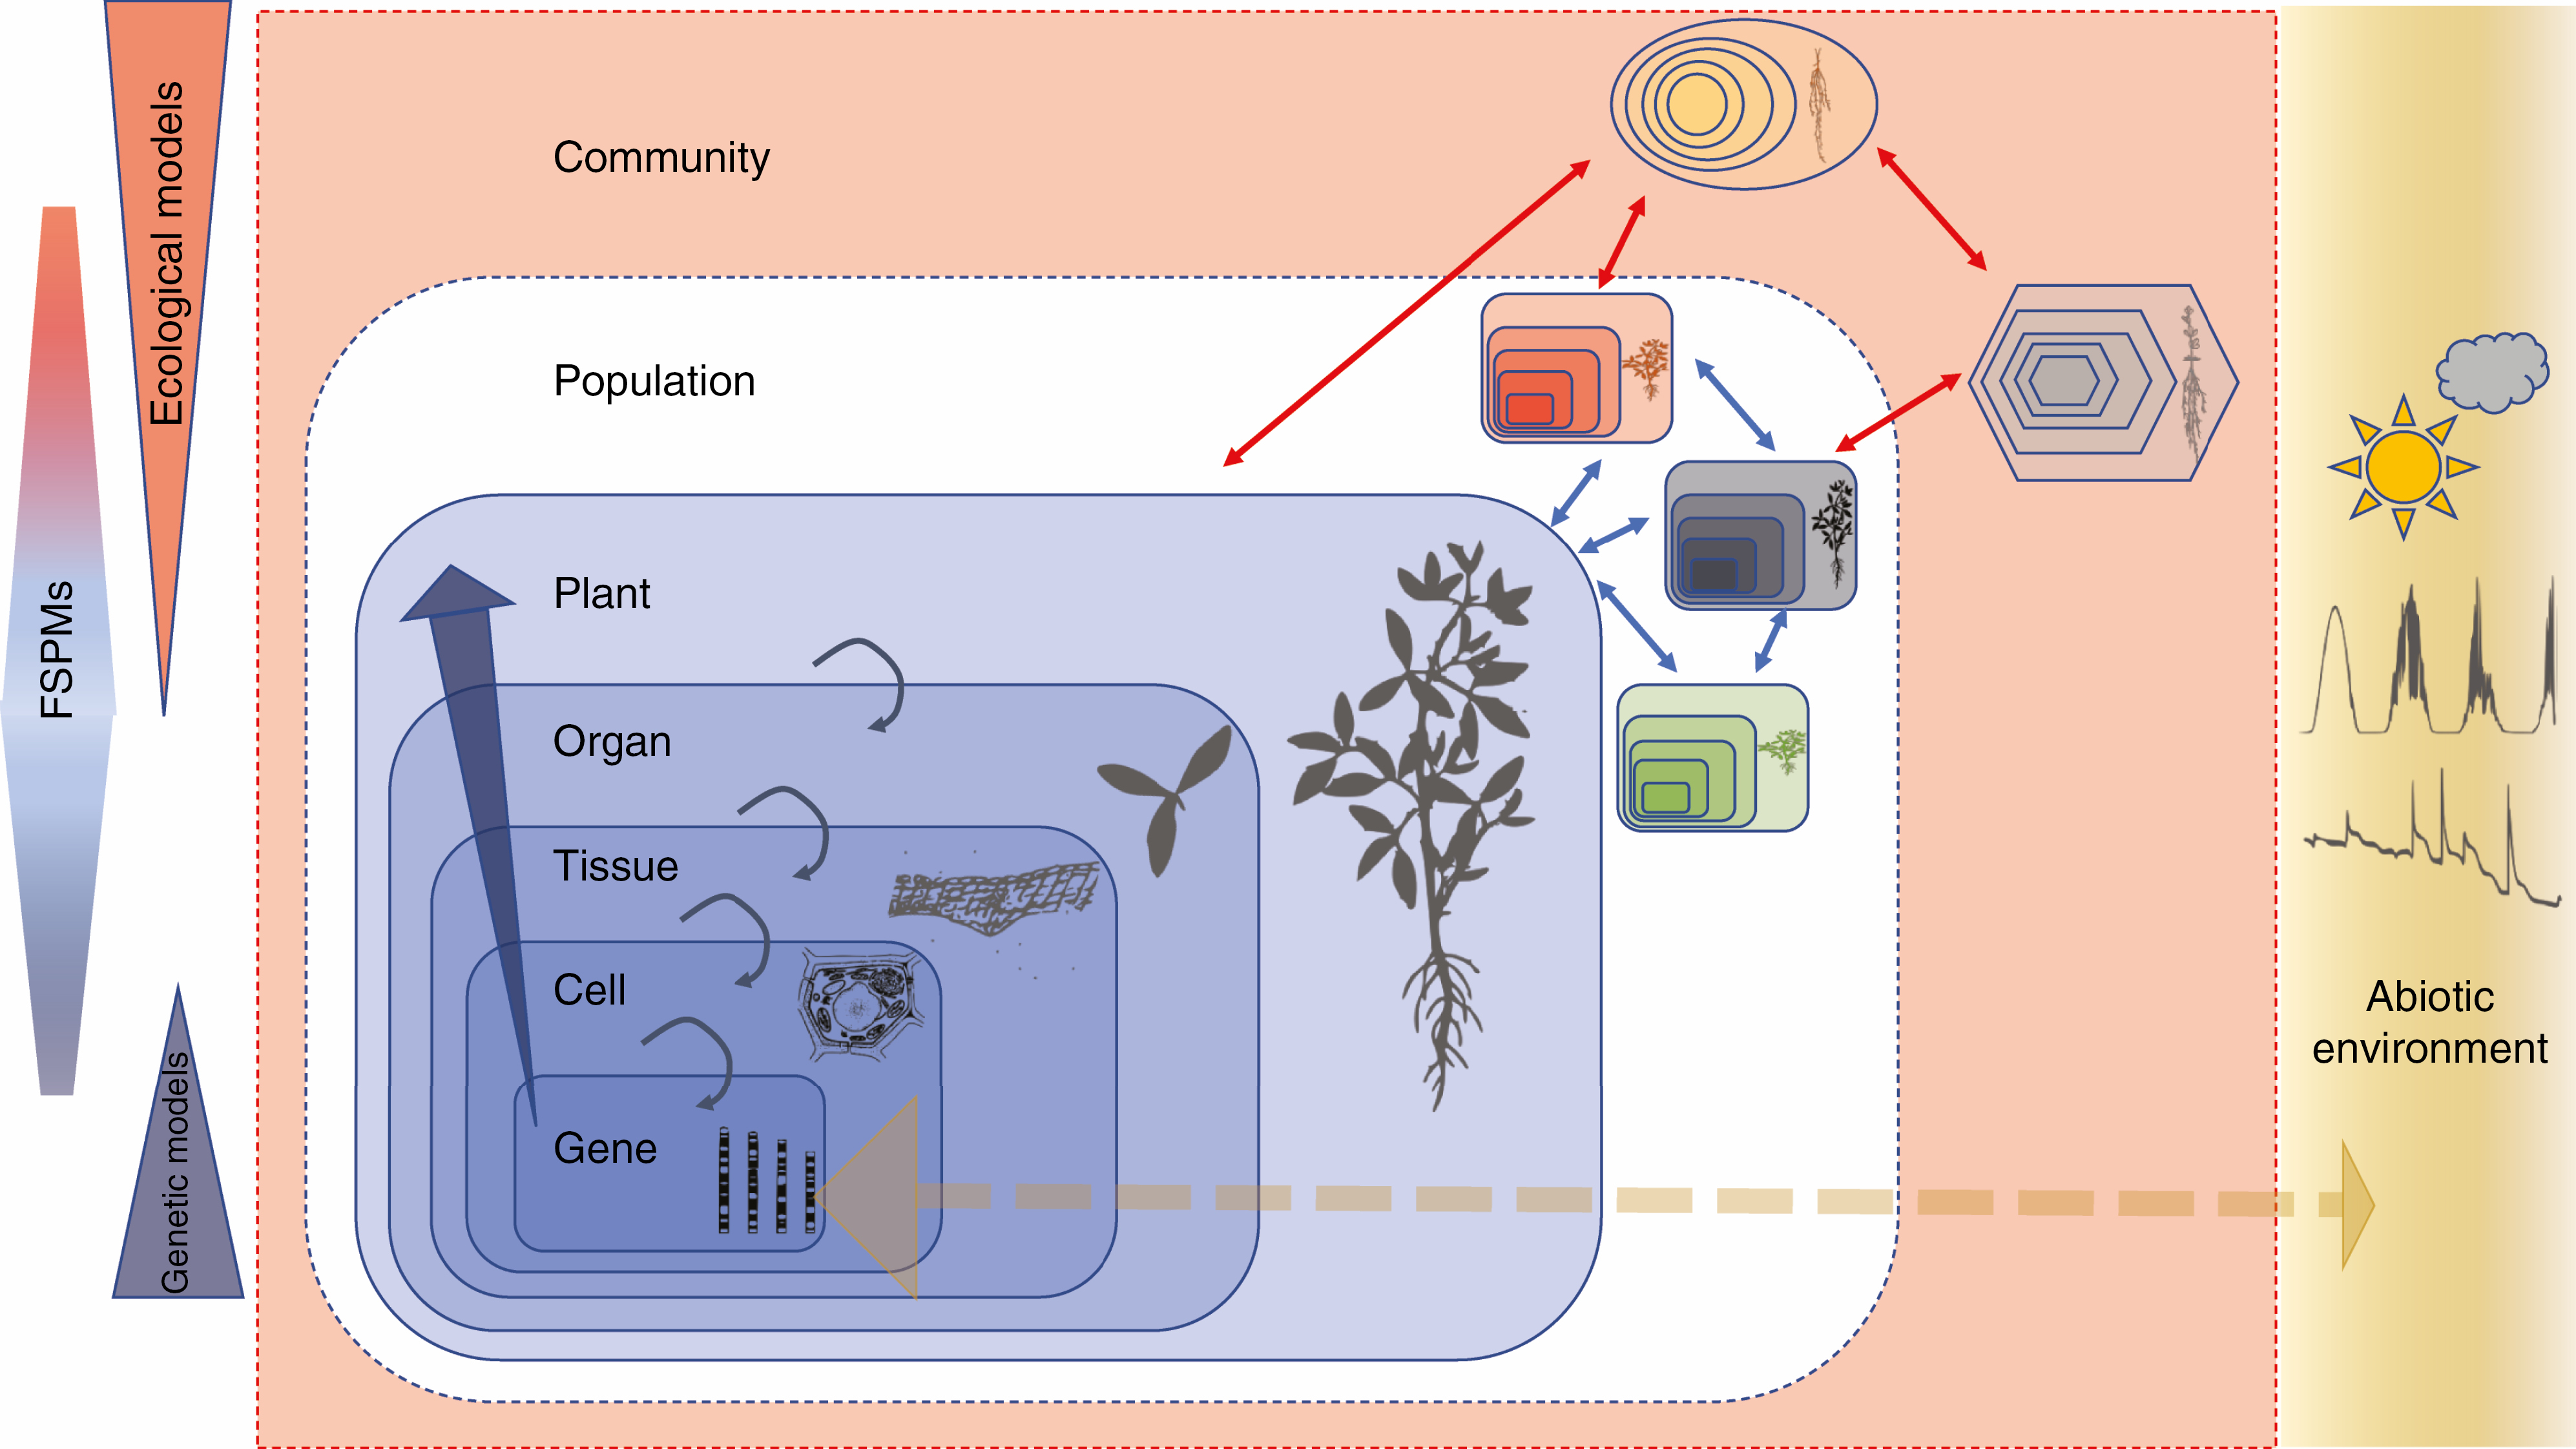
\includegraphics[width=0.8\textwidth]{img/fspm_scales_louarn_2020.jpeg}}{\textcopyright Copyright 2020 Oxford University Press}
	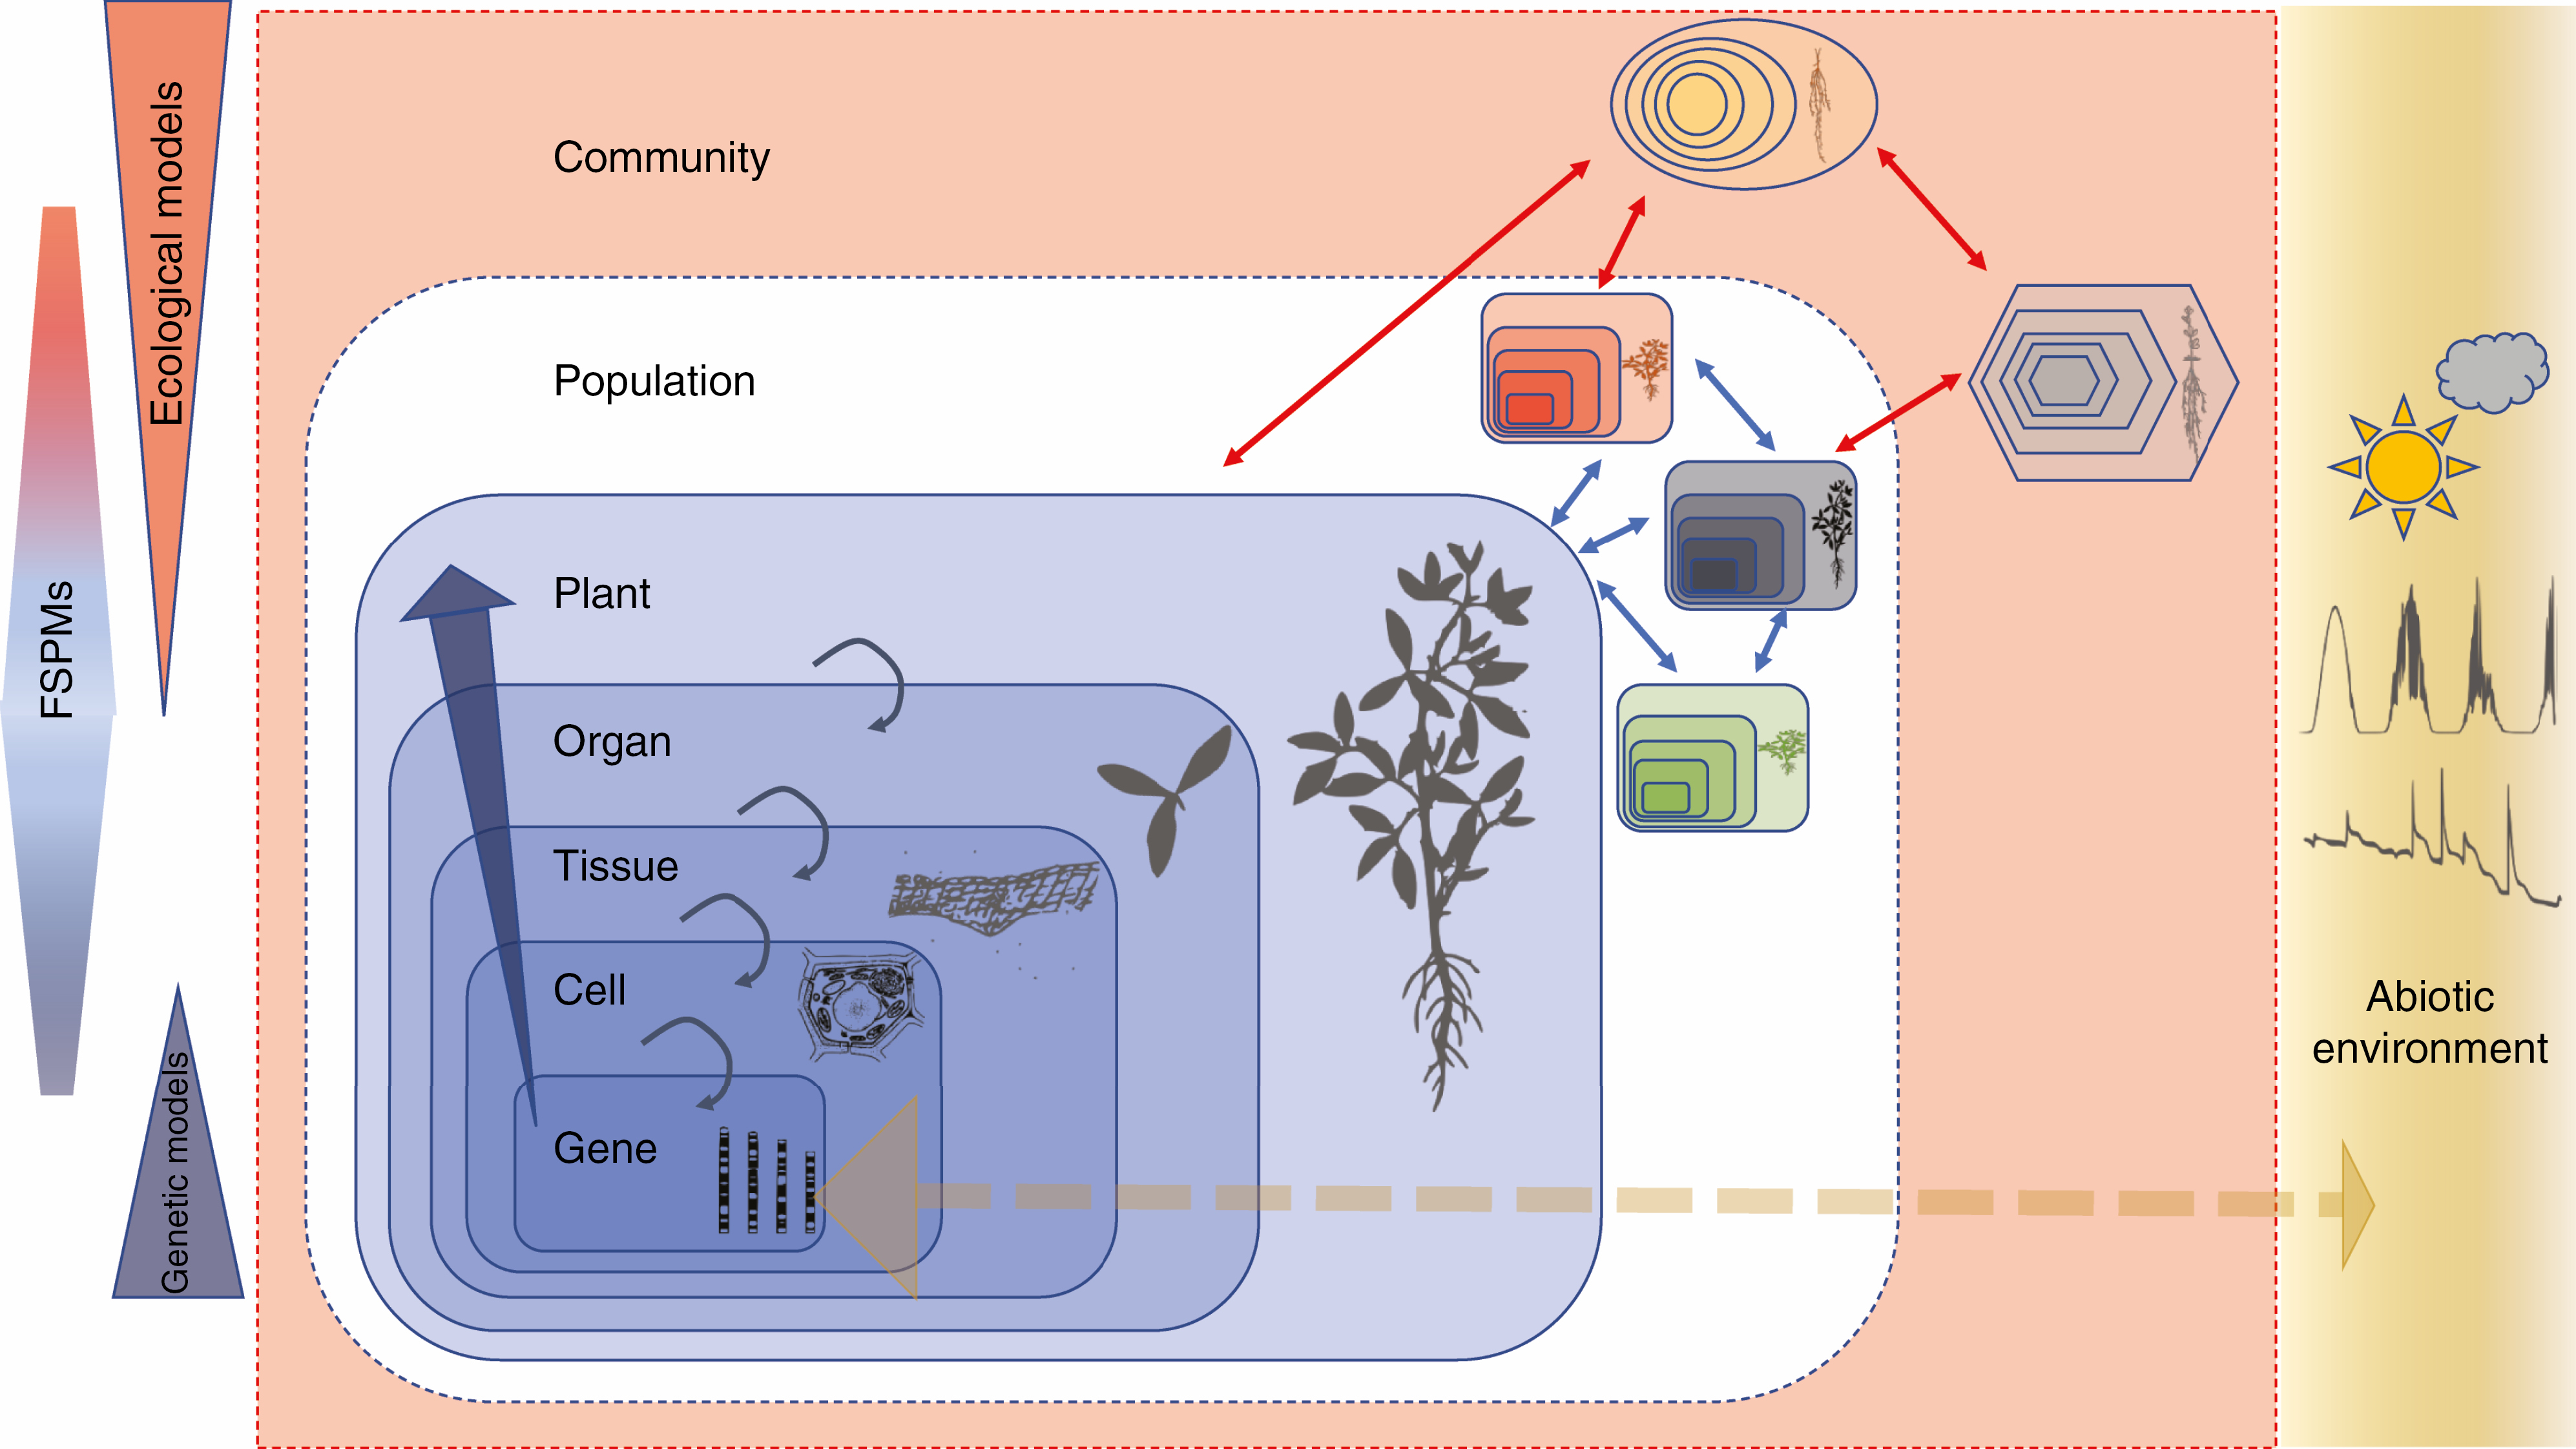
\includegraphics[width=\textwidth]{img/fspm_scales_louarn_2020.jpeg}
	
	\caption[Interactions at micro- and macroscopic scales present in functional-structural plant models (from \citet{louarn_two_2020}).]{
	        Interactions at micro- and macroscopic scales present in functional-structural plant models.
    	    \acrshort{fspm}s typically implement a subset of the scales depicted in the figure. The interactions between structural elements at one level govern the macroscopic behavior at the higher level. All levels interact with the environment. In some models, the behavior of the lowest level units is governed by variable genetic properties. This figure is reused from \citet{louarn_two_2020} with permission from the publisher.
        }
	\label{fig:fspm_scales_louarn2020}
\end{figure}


% Original caption:

% FSPMs cover a range of scale integration from gene to community level, with the focus of attention being the explanation of how plant phenotypes (centre of the figure) are built from interactions with their inner (including genetic determinants and self-regulation loops expressed at various levels) and outer (including abiotic factors and biotic interactions in plant populations and communities) environments. Interactions up to the plant scale involve sub-parts that all share the same genetic material (same shape and colour gradient in the figure) and proceed from systems biology. Interactions at higher scales integrate the interplay between entities that are genetically distinct (either from the same or different species), and contribute to predictive ecology by linking organismal traits with population and community functioning. FSPMs thus complete both classical genetic and molecular network models that are usually applied up to the cellular level, and population ecology models that are lacking a robust physiological response to environmental drivers.

% [TODO: ADD ILLUSTRATION OF FSPM]


% What are \acrshort{fspm}s for?
Functional-structural plant models owe their success to more than two decades of interdisciplinary collaboration between biology, biophysics, ecology, and computer science \citep{louarn_two_2020}.
At present, \acrshort{fspm}s have been applied in developmental biology \citep{cieslak_integrating_2016, schneider_light_2019, gauthier_functional_2020}, integrative and systems biology \citep{zhu_plants_2016, chang_systems_2019, millar_practical_2019} and applied plant sciences \citep{renton_modelling_2017, albasha_hydroshoot_2019, university_of_reading_uk_advances_2021}. 
The accelerated development in this area of research is enabled by common frameworks that standardize the description of e.g.\ plant architecture \citep{godin_multiscale_1998, boudon_l-py_2012} and eco-physiological interactions \citep{fournier_caribu_2016, zhou_cplantbox_2020}. 
Popular platforms for functional plant modelling workflows are OpenAlea \citep{pradal_openalea_2008, pradal_openalea_2015}, GroIMP \citep{vos_groimp_2007} and GreenLab \citep{de_reffye_two_2021}. 


% What do \acrshort{fspm}s model?
The precise set of simulated physiological processes varies from model to model. 
Commonly modeled factors include hydraulic pressure, water and carbon flow, and photosynthesis \citep{coussement_turgor-driven_2020, zhou_cplantbox_2020, albasha_hydroshoot_2019}. 
The complexity of the environmental simulation also differs between models, ranging from manual application of input values in root nodes \citep{zhou_cplantbox_2020} to ray-traced application of lighting conditions, including self-shading \citep{coussement_turgor-driven_2020}.
Further still, some \acrshort{fspm}s model plant growth over the span of an entire growth season \citep{lecarpentier_walter_2019, coussement_turgor-driven_2020} where others assume a static plant geometry with predefined limits for simulation duration and model accuracy \citep{albasha_hydroshoot_2019}.


% Some examples
\mbox{Figure \ref{fig:plant_model_examples}} highlights a small selection of models from the literature.
% Soybean FSPM
First, Soybean FSPM \citep{coussement_turgor-driven_2020} is a highly detailed mechanistic plant growth model. 
Soybean FSPM was developed to understand better a plant's macroscopic behavior in relation to water.
The model simulates vegetative growth driven by hydrostatic pressure inside the plant cells and incorporates a ray-traced lighting model with dynamic lighting and shading conditions \mbox{(Figure \ref{fig:fspm-soybean-fspm})}. 
% V-Mango
V-Mango \citep{boudon_v-mango_2020} models the vegatative and reproductive development of mango trees to enable \textit{in silico} experimentation with better cultivation practices.
The model allows researchers to understand why certain characteristics of mango trees make them more susceptible to pests and to study the influence of the three-dimensional tree architecture on fruit growth.
% Other models.
While this is far from an exhaustive list of what has been accomplished with FSPMs, it should give the reader an idea of what is possible with this first-principles approach to plant modeling.

\begin{figure}[t]
    \centering
    \begin{subfigure}[b]{0.48\linewidth}
        \centering
        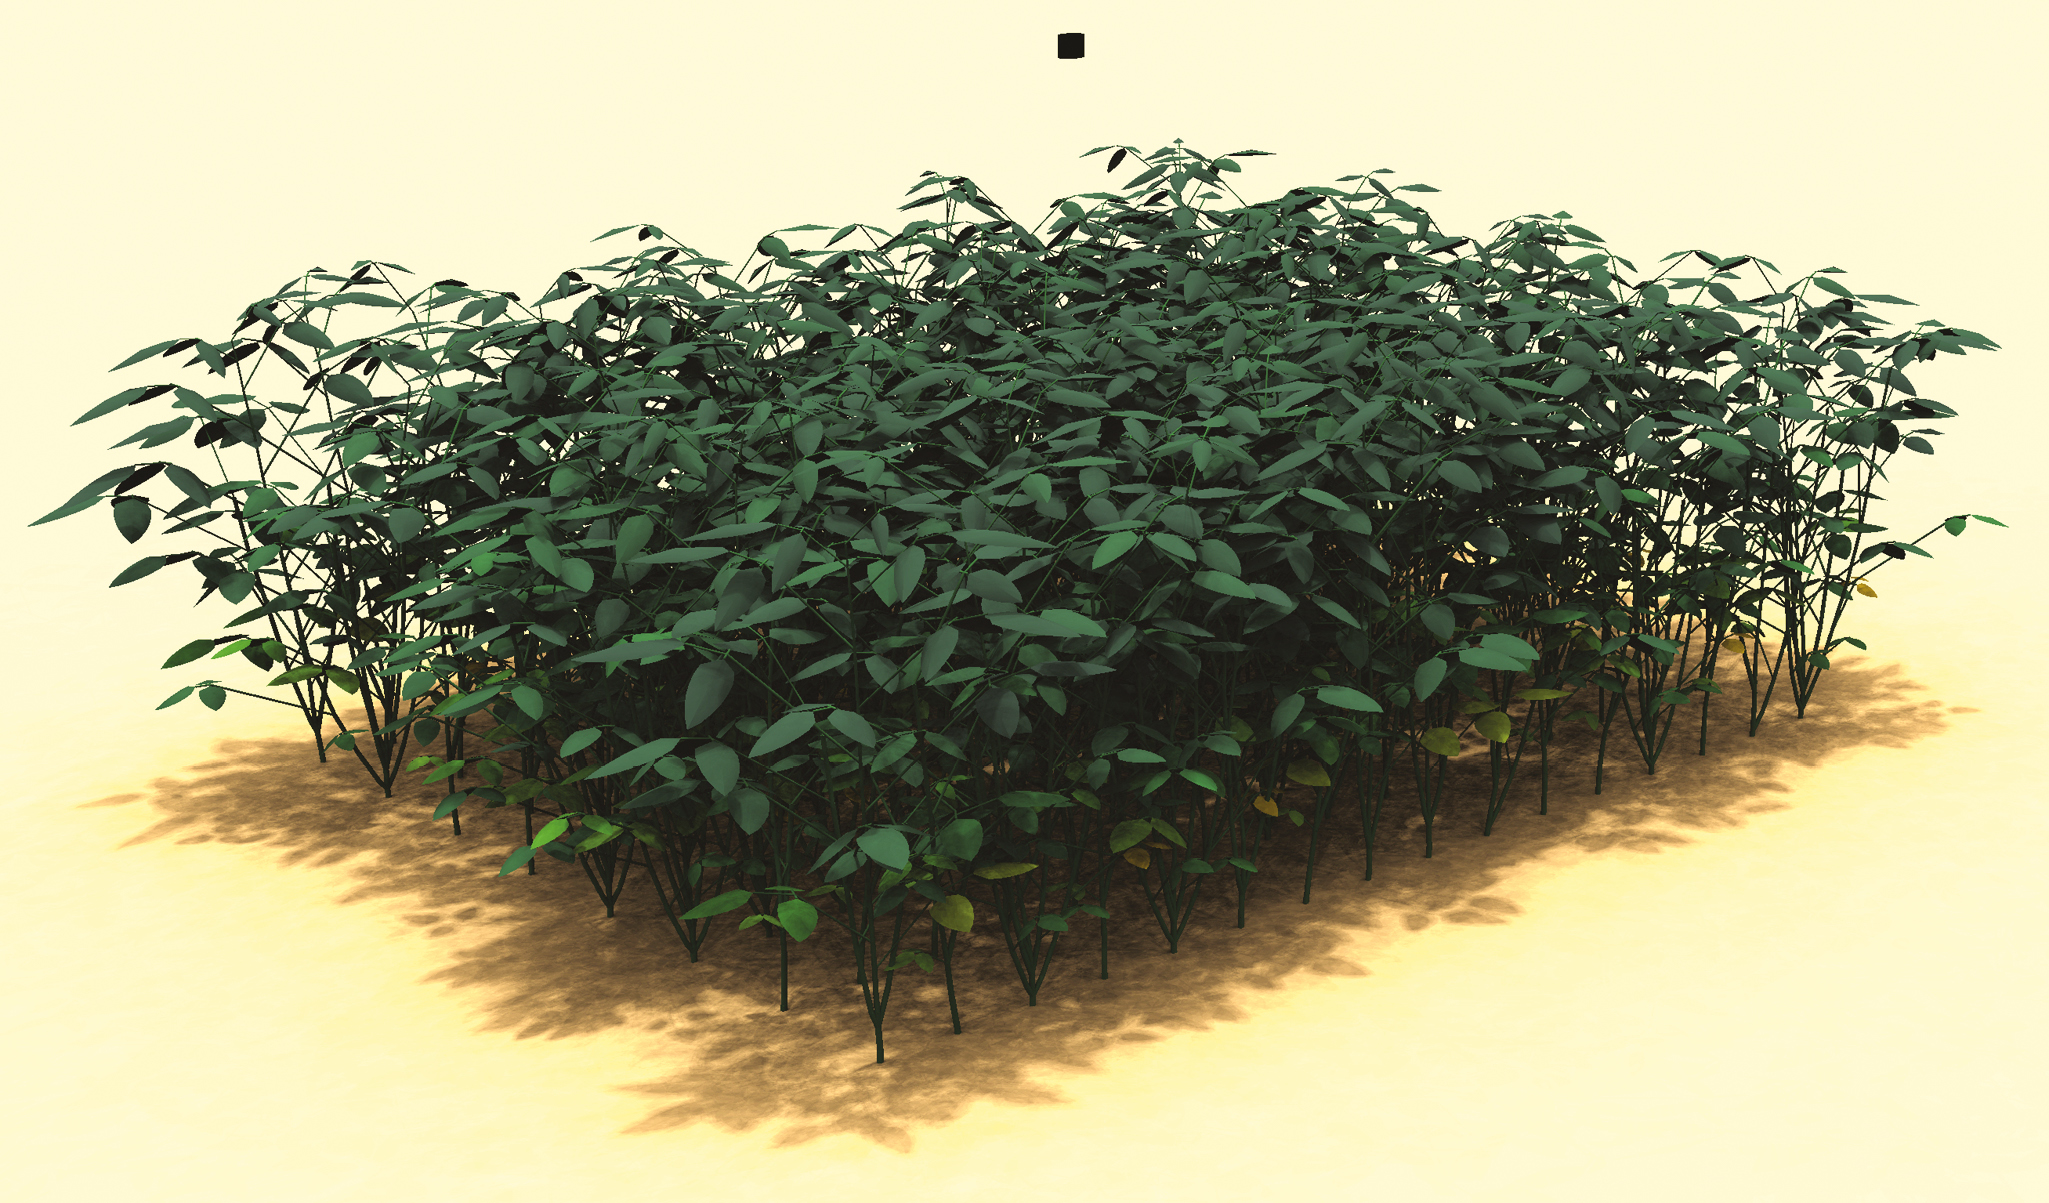
\includegraphics[width=\linewidth,height=\linewidth,keepaspectratio]{img/soybean_canopy_coussement.jpeg}
        \caption{Soybean FSPM}
        \label{fig:fspm-soybean-fspm}
    \end{subfigure}
    \hfill
    \begin{subfigure}[b]{0.48\linewidth}
        \centering
        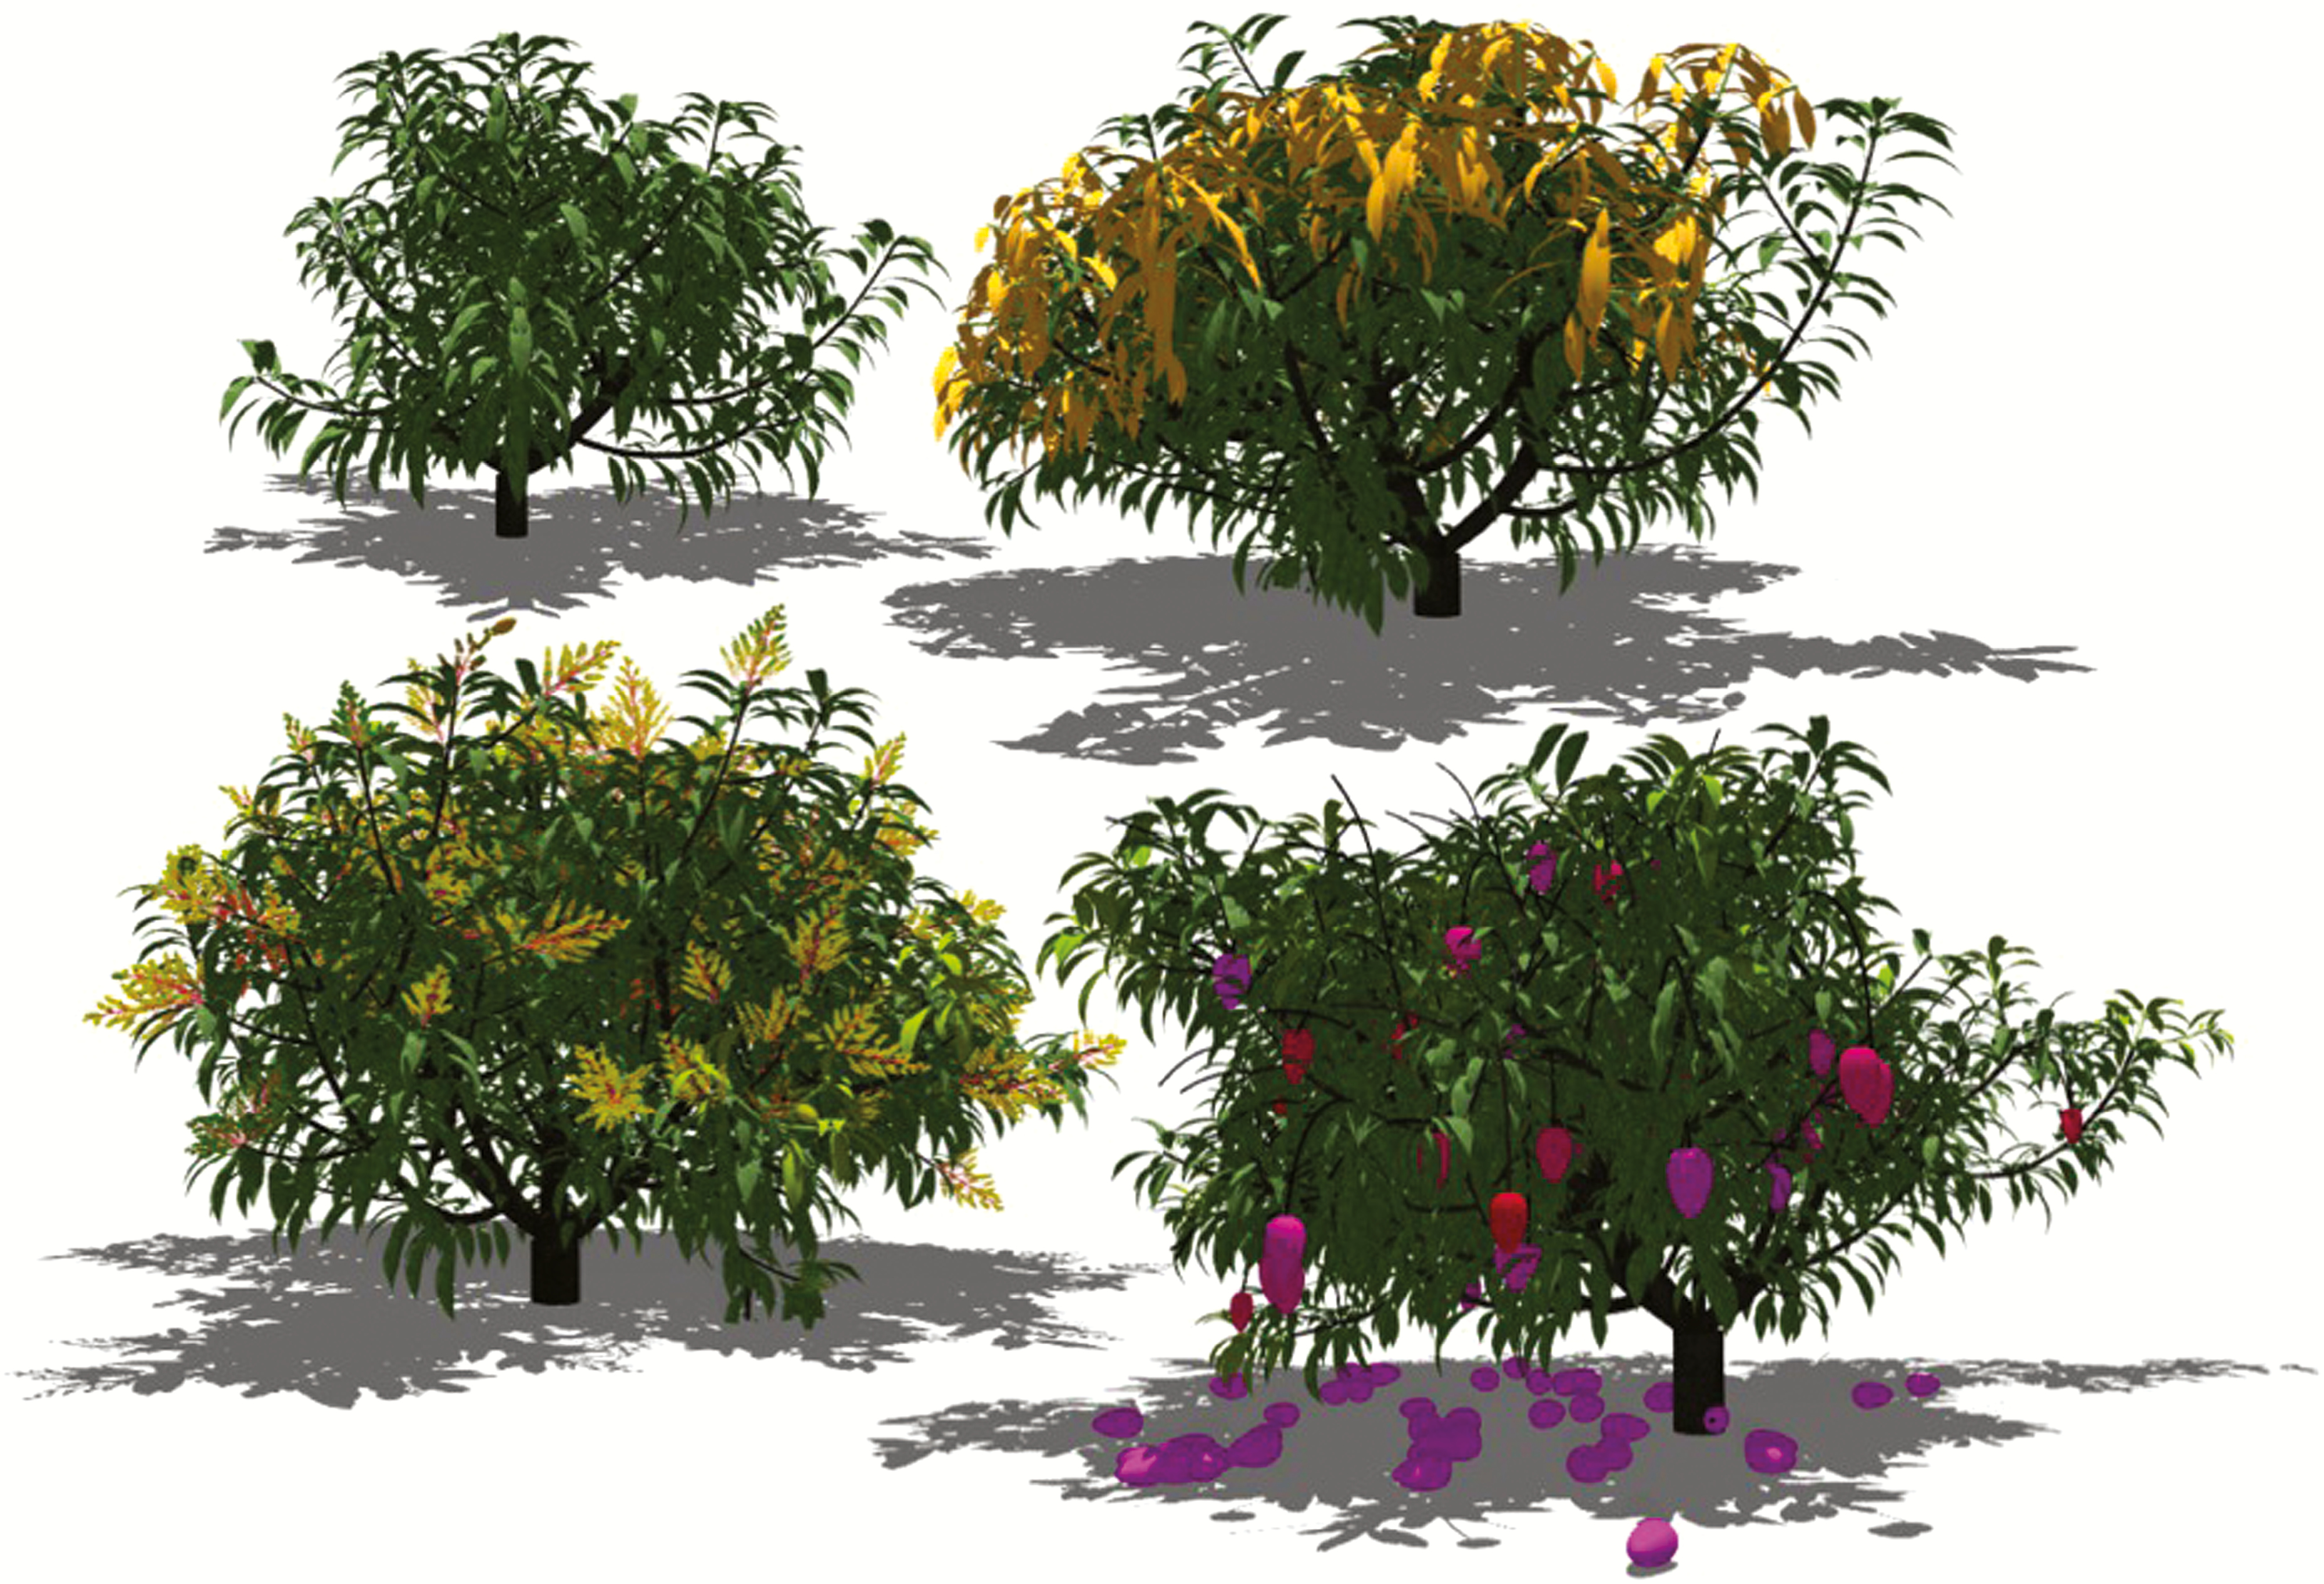
\includegraphics[width=\linewidth,height=\linewidth,keepaspectratio]{img/vmango_example.jpeg}
        \caption{V-Mango}
        \label{fig:fspm-vmango}
    \end{subfigure}
    % \vskip\baselineskip
    % \begin{subfigure}[b]{0.45\linewidth}
    %     \centering
    %     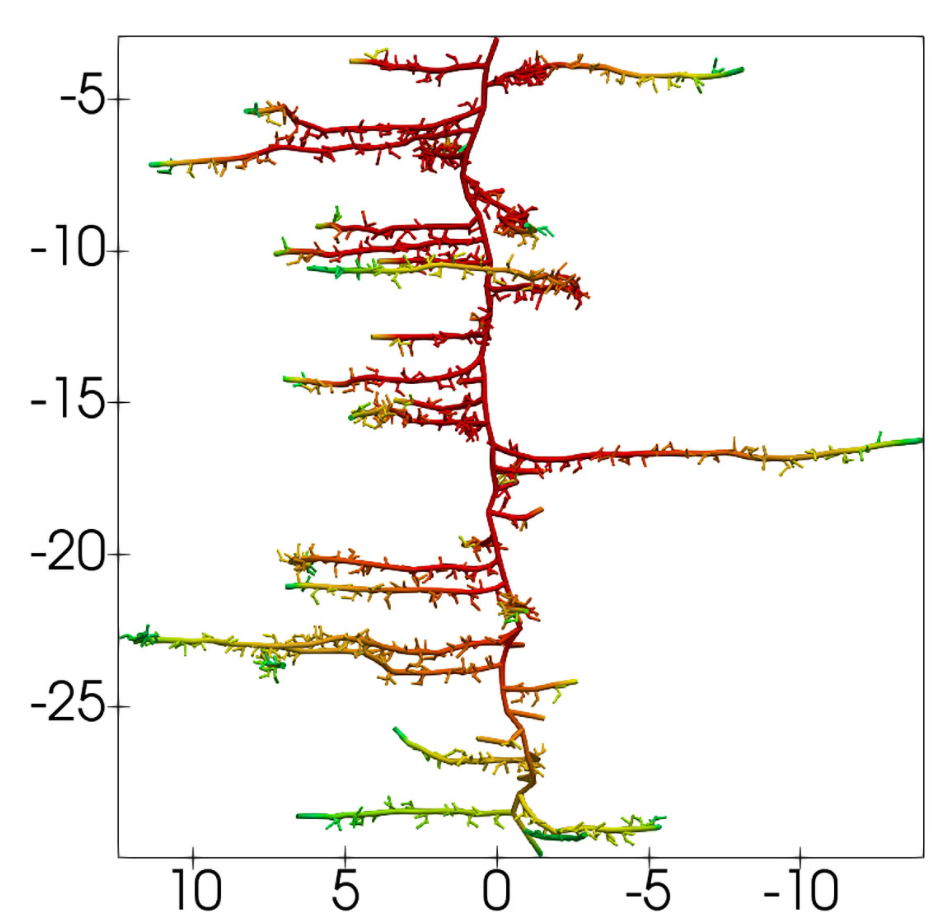
\includegraphics[width=\linewidth,height=\linewidth,keepaspectratio]{img/crootbox_example_anagallis_femina.png}
    %     \caption{CRootBox}
    %     \label{fig:fspm-crootbox}
    % \end{subfigure}
    % \hfill
    % \begin{subfigure}[b]{0.45\linewidth}
    %     \centering
    %     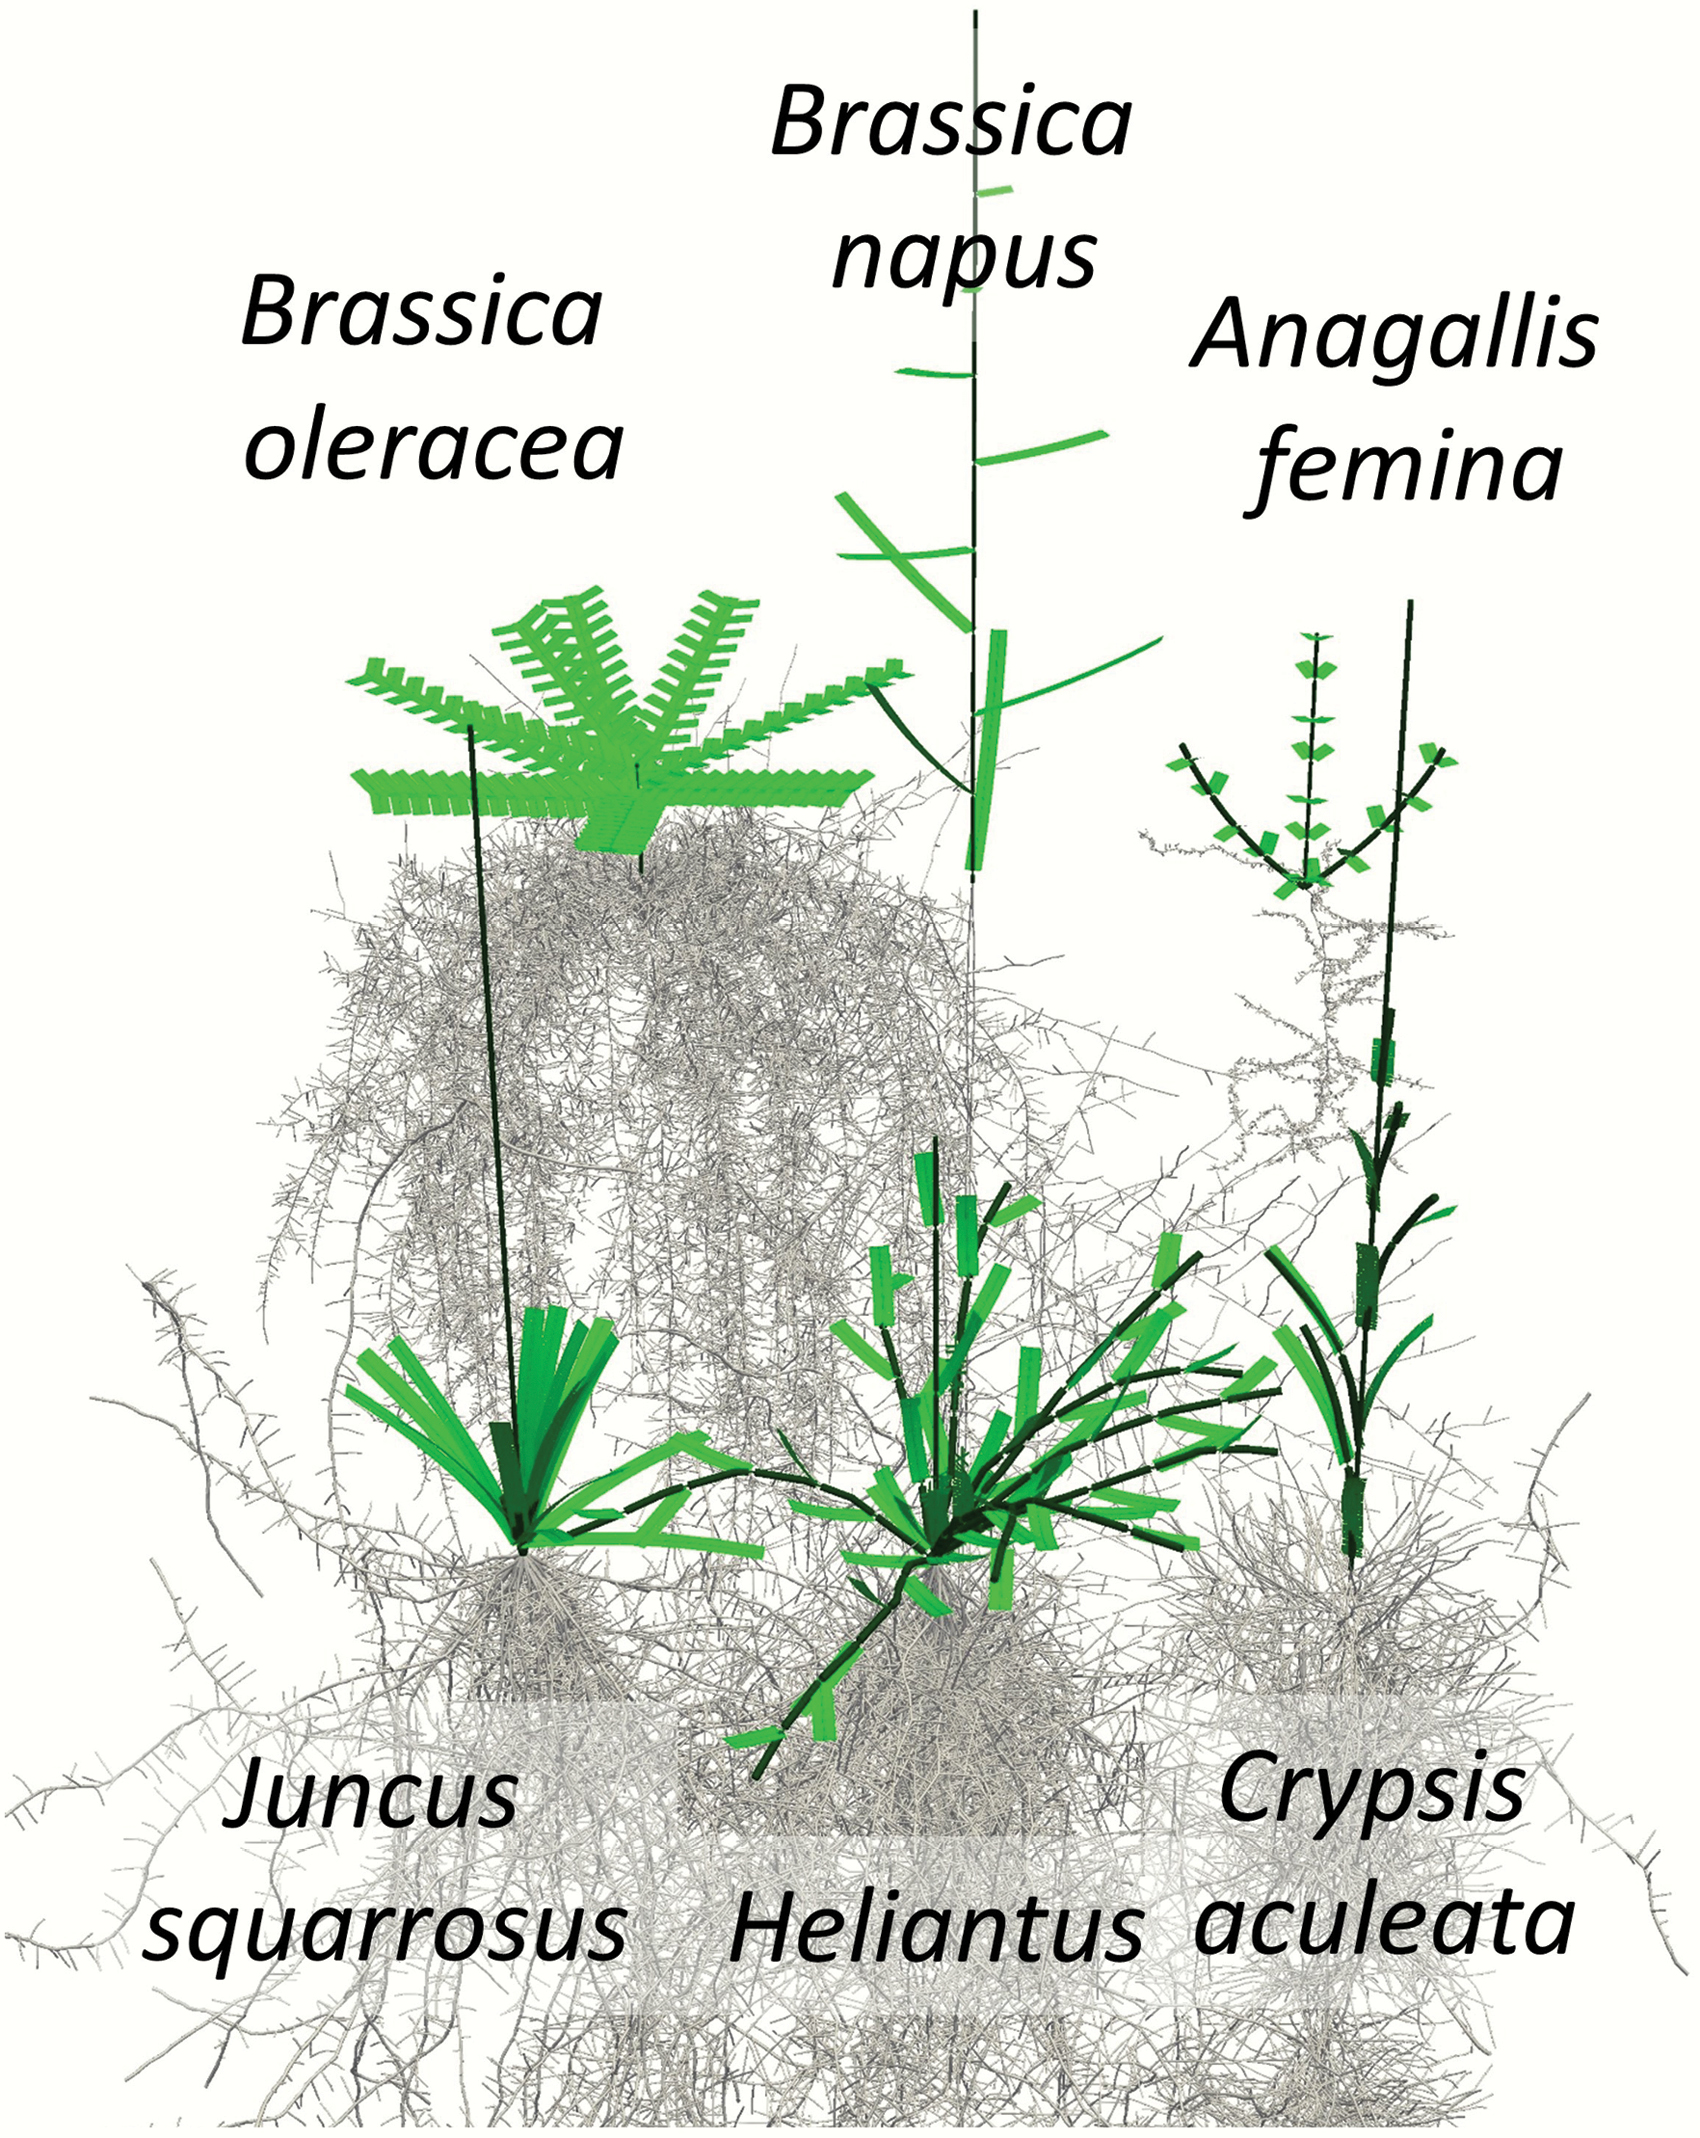
\includegraphics[width=\linewidth,height=\linewidth,keepaspectratio]{img/cplantbox_example.jpeg}
    %     \caption{CPlantBox}
    %     \label{fig:fspm-cplantbox}
    % \end{subfigure}
    \caption[Two examples of functional-structural plant models.]{
            Two examples of functional-structural plant models. 
            % (\subref{fig:fspm-soybean-fspm}) Soybean FSPM \supercite{coussement_turgor-driven_2020} is a highly detailed mechanistic plant growth model driven by hydrostatic pressure inside the plant cells. It also incorporates a ray-traced lighting model with dynamic lighting and shading conditions. 
            % (\subref{fig:fspm-vmango}) V-Mango \supercite{boudon_v-mango_2020} models the vegatative and reproductive development of mango trees to enable \textit{in silico} experimentation with better cultivation practices.
            % (\subref{fig:fspm-crootbox}) CRootBox \supercite{schnepf_crootbox_2018} is a generic framework for modeling the growth of plant roots in varying soil and environmental conditions.
            % (\subref{fig:fspm-cplantbox}) CPlantBox \supercite{zhou_cplantbox_2020} is built on top of CRootBox to provide a generic framework for modeling plant architecture and growth. It can be coupled with existing simulations of eco-physiological processes to create mechanistic plant models. 
            Figures originally appeared in their respective cited works.
            (\subref{fig:fspm-soybean-fspm}) Soybean FSPM \citep{coussement_turgor-driven_2020}. Figure reused with permission from the publisher (Copyright 2018 Oxford University Press).
            (\subref{fig:fspm-soybean-fspm}) V-Mango \citep{boudon_v-mango_2020}. Figure reused under the CC BY 4.0 license.
    }
    \label{fig:plant_model_examples}
\end{figure}

% (Coussement et al. 2018\supercite{coussement_modelling_2018})



% Caution before reusing an FSPM from the literature
An important caveat is that these models typically do not simulate a live plant as an accurate digital twin of an \textit{in vivo} plant.
Instead, they are commonly developed with a specific research question in mind and model only the physiological processes that are deemed correlated to the studied phenomenon \citep{louarn_two_2020}.
Hence, it is warranted to perform a careful comparison between the conditions and assumptions of the original study and those of a new context before reusing the model for tasks other than its original purpose.
Note that digital twin initiatives are also an active line of research. For example, researchers at WUR have been developing a digital twin system for tomato plants \citep{npec_wur_2020}.


% \section{Related work} \label{fspm:related}

% % interdisciplinary collaboration

FSPMs owe their success to more than two decades of interdisciplinary collaboration between biology, biophysics, ecology and computer science \supercite{louarn_two_2020}.


% Cite that frameworks have made it easier to iterate and build on existing work and cite some frameworks
%  	- MTG OpenAlea, LPy,  CPlantBox, GroIMP, GreenLab, 

...

% give examples of some noteable works (use [[@louarnTwoDecadesFunctional2020]] as a guide for finding good citations)

...

% Useful citations: OpenAlea platform \cite{pradal_openalea_2008, pradal_openalea_2015}, LPy for L-systems in Python \cite{boudon_l-py_2012}, CPlantBox \cite{zhou_cplantbox_2020}, GroIMP \cite{citation needed}, GreenLab \cite{de_reffye_two_2021}, ...



% \cite{balduzzi_reshaping_2017}, popular data structure MTG \cite{godin_multiscale_1998}

\section{Summary}

This chapter introduced the research field of functional-structural plant modeling, a type of model that has become the state-of-the-art in plant modeling in the past years.
FSPMs represent the plant as a 3D structure of interconnected elements, where each structural element simulates eco-physiological processes such as photosynthesis, transpiration, and water and carbon flow.
FSPMs are ideal for reservoir computing research because they model the interaction in space and time between the plant's structure and the abiotic environment.
Therefore, if plant physiology displays properties of nonlinear dynamical systems, this will be captured by a sufficiently detailed FSPM.